\documentclass[12pt,letterpaper]{article}\usepackage[]{graphicx}\usepackage[]{color}
%% maxwidth is the original width if it is less than linewidth
%% otherwise use linewidth (to make sure the graphics do not exceed the margin)
\makeatletter
\def\maxwidth{ %
  \ifdim\Gin@nat@width>\linewidth
    \linewidth
  \else
    \Gin@nat@width
  \fi
}
\makeatother

\definecolor{fgcolor}{rgb}{0.345, 0.345, 0.345}
\newcommand{\hlnum}[1]{\textcolor[rgb]{0.686,0.059,0.569}{#1}}%
\newcommand{\hlstr}[1]{\textcolor[rgb]{0.192,0.494,0.8}{#1}}%
\newcommand{\hlcom}[1]{\textcolor[rgb]{0.678,0.584,0.686}{\textit{#1}}}%
\newcommand{\hlopt}[1]{\textcolor[rgb]{0,0,0}{#1}}%
\newcommand{\hlstd}[1]{\textcolor[rgb]{0.345,0.345,0.345}{#1}}%
\newcommand{\hlkwa}[1]{\textcolor[rgb]{0.161,0.373,0.58}{\textbf{#1}}}%
\newcommand{\hlkwb}[1]{\textcolor[rgb]{0.69,0.353,0.396}{#1}}%
\newcommand{\hlkwc}[1]{\textcolor[rgb]{0.333,0.667,0.333}{#1}}%
\newcommand{\hlkwd}[1]{\textcolor[rgb]{0.737,0.353,0.396}{\textbf{#1}}}%

\usepackage{framed}
\makeatletter
\newenvironment{kframe}{%
 \def\at@end@of@kframe{}%
 \ifinner\ifhmode%
  \def\at@end@of@kframe{\end{minipage}}%
  \begin{minipage}{\columnwidth}%
 \fi\fi%
 \def\FrameCommand##1{\hskip\@totalleftmargin \hskip-\fboxsep
 \colorbox{shadecolor}{##1}\hskip-\fboxsep
     % There is no \\@totalrightmargin, so:
     \hskip-\linewidth \hskip-\@totalleftmargin \hskip\columnwidth}%
 \MakeFramed {\advance\hsize-\width
   \@totalleftmargin\z@ \linewidth\hsize
   \@setminipage}}%
 {\par\unskip\endMakeFramed%
 \at@end@of@kframe}
\makeatother

\definecolor{shadecolor}{rgb}{.97, .97, .97}
\definecolor{messagecolor}{rgb}{0, 0, 0}
\definecolor{warningcolor}{rgb}{1, 0, 1}
\definecolor{errorcolor}{rgb}{1, 0, 0}
\newenvironment{knitrout}{}{} % an empty environment to be redefined in TeX

\usepackage{alltt}
 \usepackage[left=2cm,right=2cm,top=2cm,bottom=2cm]{geometry}
\usepackage[ansinew]{inputenc}
\usepackage[spanish]{babel}
\usepackage{amsmath}
\usepackage{amsfonts}
\usepackage{amssymb}
\usepackage{dsfont}
\usepackage{multicol} 
\usepackage{subfigure}
\usepackage{graphicx}
\usepackage{float} 
\usepackage{verbatim} 
\usepackage[left=2cm,right=2cm,top=2cm,bottom=2cm]{geometry}
\usepackage{fancyhdr}
\pagestyle{fancy} 
\fancyhead[LO]{\leftmark}
\usepackage{caption}
\newtheorem{definicion}{Definci\'on}
\IfFileExists{upquote.sty}{\usepackage{upquote}}{}
\begin{document}

\begin{titlepage}
\setlength{\unitlength}{1 cm} %Especificar unidad de trabajo


\begin{center}
\textbf{{\large UNIVERSIDAD DE EL SALVADOR}\\
{\large FACULTAD MULTIDISCIPLINARIA DE OCCIDENTE}\\
{\large DEPARTAMENTO DE MATEM\'ATICA}}\\[0.50 cm]

\begin{picture}(18,4)
 \put(7,0){
\includegraphics[width=4cm]{minerva.jpg}}
\end{picture}
\\[0.25 cm]

\textbf{{\large Licenciatura en Estad\'istica}\\[1.25cm]
{\large Control Estadistico del Paquete R }\\[2 cm]
%\setlength{\unitlength}{1 cm}
{\large  \textbf{''UNIDAD DOS"}}\\
{\large  \textbf{Pr\'actica 11-An\'alisis de una variable bidimensional cuantitativa }}\\[3 cm]
{\large Alumna:}\\
{\large Martha Yoana Medina S\'anchez}\\[2cm]
{\large Fecha de elaboraci\'on}\\
Santa Ana - \today }
\end{center}
\end{titlepage}

\newtheorem{teorema}{Teorema}
\newtheorem{prop}{Proposici\'on}[section]

\lhead{UNIDAD DOS}
\chead{PR\'ACTICA 11}
\lfoot{LICENCIATURA EN ESTAD\'ISTICA}
\cfoot{UESOCC}
\rfoot{\thepage}
%\pagestyle{fancy} 

\setcounter{page}{1}
\newpage


\begin{center}
\subsubsection*{Pr\'actica 11-An\'alisis de una variable bidimensional cuantitativa}
\subsection*{REALICE UN AN\'ALISIS ESTAD\'ISTICO.}
\end{center}

\subsection*{EJEMPLO}

\begin{enumerate}
\item Activa tu directorio de trabajo 

\begin{knitrout}
\definecolor{shadecolor}{rgb}{0.969, 0.969, 0.969}\color{fgcolor}\begin{kframe}
\begin{alltt}
\hlkwd{getwd}\hlstd{()}
\end{alltt}
\begin{verbatim}
## [1] "C:/Users/User/Documents/PRACTICAS_YOANA_MEDINA/Yoana/PRACTICAS DE R"
\end{verbatim}
\begin{alltt}
\hlkwd{setwd}\hlstd{(}\hlstr{"C:/Users/User/Documents/PRACTICAS_YOANA_MEDINA/Yoana/PRACTICAS DE R"}\hlstd{)}
\end{alltt}
\end{kframe}
\end{knitrout}

\item Crea un nuevo script y ll\'amale "Script11-DatosBivariados4" 

\item Crea los dos vectores para las dos variables 

\begin{knitrout}
\definecolor{shadecolor}{rgb}{0.969, 0.969, 0.969}\color{fgcolor}\begin{kframe}
\begin{alltt}
\hlcom{# Numero de usuarios = Variable explicativa o independiente}

\hlstd{usuarios} \hlkwb{<-} \hlkwd{c}\hlstd{(}\hlnum{10}\hlstd{,} \hlnum{15}\hlstd{,} \hlnum{20}\hlstd{,} \hlnum{20}\hlstd{,} \hlnum{25}\hlstd{,} \hlnum{30}\hlstd{,} \hlnum{30}\hlstd{); usuarios}
\end{alltt}
\begin{verbatim}
## [1] 10 15 20 20 25 30 30
\end{verbatim}
\begin{alltt}
\hlstd{tiempo} \hlkwb{=} \hlkwd{c}\hlstd{(}\hlnum{1.0}\hlstd{,} \hlnum{1.2}\hlstd{,} \hlnum{2.0}\hlstd{,} \hlnum{2.1}\hlstd{,} \hlnum{2.2}\hlstd{,} \hlnum{2.0}\hlstd{,} \hlnum{1.9}\hlstd{); tiempo}
\end{alltt}
\begin{verbatim}
## [1] 1.0 1.2 2.0 2.1 2.2 2.0 1.9
\end{verbatim}
\end{kframe}
\end{knitrout}

\item Crea una hoja de datos que tenga como componentes o columnas los dos vectores.

\begin{knitrout}
\definecolor{shadecolor}{rgb}{0.969, 0.969, 0.969}\color{fgcolor}\begin{kframe}
\begin{alltt}
\hlstd{Sistema} \hlkwb{<-} \hlkwd{data.frame}\hlstd{(}\hlkwc{Usuarios}\hlstd{=usuarios,} \hlkwc{Tiempo}\hlstd{=tiempo);Sistema}
\end{alltt}
\begin{verbatim}
##   Usuarios Tiempo
## 1       10    1.0
## 2       15    1.2
## 3       20    2.0
## 4       20    2.1
## 5       25    2.2
## 6       30    2.0
## 7       30    1.9
\end{verbatim}
\begin{alltt}
\hlcom{# Para editar o ampliar los datos puede utilizar la función fix() }

\hlkwd{fix}\hlstd{(Sistema)}
\end{alltt}
\end{kframe}
\end{knitrout}

\item Guarda la hoja de datos en un archivo. 

\begin{knitrout}
\definecolor{shadecolor}{rgb}{0.969, 0.969, 0.969}\color{fgcolor}\begin{kframe}
\begin{alltt}
\hlkwd{write.table}\hlstd{(Sistema,} \hlkwc{file}\hlstd{=}\hlstr{"Sistema.txt"}\hlstd{,} \hlkwc{append}\hlstd{=}\hlnum{FALSE}\hlstd{,} \hlkwc{quote}\hlstd{=}\hlnum{TRUE}\hlstd{,}
            \hlkwc{sep}\hlstd{=}\hlstr{" "}\hlstd{,} \hlkwc{na}\hlstd{=}\hlstr{"NA"}\hlstd{,} \hlkwc{col.names} \hlstd{=} \hlnum{TRUE}\hlstd{)}
\end{alltt}
\end{kframe}
\end{knitrout}

\item Elimina los objetos almacenados en el \'area de trabajo (Workspace).

\begin{knitrout}
\definecolor{shadecolor}{rgb}{0.969, 0.969, 0.969}\color{fgcolor}\begin{kframe}
\begin{alltt}
\hlkwd{ls}\hlstd{();}
\end{alltt}
\begin{verbatim}
## [1] "Sistema"  "tiempo"   "usuarios"
\end{verbatim}
\begin{alltt}
\hlkwd{rm}\hlstd{(}\hlkwc{list}\hlstd{=}\hlkwd{ls}\hlstd{(}\hlkwc{all}\hlstd{=}\hlnum{TRUE}\hlstd{));}
\hlkwd{ls}\hlstd{()}
\end{alltt}
\begin{verbatim}
## character(0)
\end{verbatim}
\end{kframe}
\end{knitrout}

\item Recupera la hoja de datos. 
  
\begin{knitrout}
\definecolor{shadecolor}{rgb}{0.969, 0.969, 0.969}\color{fgcolor}\begin{kframe}
\begin{alltt}
\hlstd{Sistema} \hlkwb{<-} \hlkwd{read.table}\hlstd{(}\hlstr{"Sistema.txt"}\hlstd{,} \hlkwc{header}\hlstd{=}\hlnum{TRUE}\hlstd{); Sistema}
\end{alltt}
\begin{verbatim}
##   Usuarios Tiempo
## 1       10    1.0
## 2       15    1.2
## 3       20    2.0
## 4       20    2.1
## 5       25    2.2
## 6       30    2.0
## 7       30    1.9
\end{verbatim}
\end{kframe}
\end{knitrout}

\item Conecta la hoja de datos a la segunda ruta o lista de b\'usqueda.

\begin{knitrout}
\definecolor{shadecolor}{rgb}{0.969, 0.969, 0.969}\color{fgcolor}\begin{kframe}
\begin{alltt}
\hlkwd{attach}\hlstd{(Sistema,} \hlkwc{pos}\hlstd{=}\hlnum{2}\hlstd{);} \hlkwd{search}\hlstd{()}
\end{alltt}
\begin{verbatim}
##  [1] ".GlobalEnv"        "Sistema"           "package:knitr"    
##  [4] "package:stats"     "package:graphics"  "package:grDevices"
##  [7] "package:utils"     "package:datasets"  "package:methods"  
## [10] "Autoloads"         "package:base"
\end{verbatim}
\end{kframe}
\end{knitrout}

\item Muestra un resumen de principales estad\'isticos de las variables.

\begin{knitrout}
\definecolor{shadecolor}{rgb}{0.969, 0.969, 0.969}\color{fgcolor}\begin{kframe}
\begin{alltt}
\hlkwd{summary}\hlstd{(Sistema)}
\end{alltt}
\begin{verbatim}
##     Usuarios         Tiempo     
##  Min.   :10.00   Min.   :1.000  
##  1st Qu.:17.50   1st Qu.:1.550  
##  Median :20.00   Median :2.000  
##  Mean   :21.43   Mean   :1.771  
##  3rd Qu.:27.50   3rd Qu.:2.050  
##  Max.   :30.00   Max.   :2.200
\end{verbatim}
\begin{alltt}
\hlkwd{cov}\hlstd{(Sistema)} \hlcom{# Matriz de covarianzas }
\end{alltt}
\begin{verbatim}
##           Usuarios   Tiempo
## Usuarios 55.952381 2.714286
## Tiempo    2.714286 0.222381
\end{verbatim}
\begin{alltt}
\hlkwd{cor}\hlstd{(Sistema,} \hlkwc{use} \hlstd{=} \hlstr{"all.obs"}\hlstd{,} \hlkwc{method}\hlstd{=}\hlstr{"pearson"}\hlstd{)}
\end{alltt}
\begin{verbatim}
##           Usuarios    Tiempo
## Usuarios 1.0000000 0.7694803
## Tiempo   0.7694803 1.0000000
\end{verbatim}
\begin{alltt}
\hlcom{# Matriz de correlaciones }
\end{alltt}
\end{kframe}
\end{knitrout}

\item Elabora un gr\'afico de dispersi\'on para analizar alguna relaci\'on entre las variables.  

\begin{knitrout}
\definecolor{shadecolor}{rgb}{0.969, 0.969, 0.969}\color{fgcolor}\begin{kframe}
\begin{alltt}
\hlkwd{plot}\hlstd{(Usuarios, Tiempo,} \hlkwc{xlim}\hlstd{=} \hlkwd{c}\hlstd{(}\hlnum{5}\hlstd{,} \hlnum{35}\hlstd{),} \hlkwc{ylim}\hlstd{=} \hlkwd{c}\hlstd{(}\hlnum{0.0}\hlstd{,} \hlnum{2.5}\hlstd{),}
\hlkwc{type} \hlstd{=} \hlstr{"p"}\hlstd{,} \hlkwc{pch}\hlstd{=}\hlnum{1}\hlstd{,} \hlkwc{col} \hlstd{=} \hlstr{"blue"}\hlstd{,} \hlkwc{main} \hlstd{=} \hlstr{"Gráfico de dispersión 
(Usuarios, Tiempo)"}\hlstd{,} \hlkwc{xlab}\hlstd{=}\hlstr{"Número de usuarios"}\hlstd{,} \hlkwc{ylab}\hlstd{=}\hlstr{"Tiempo de 
ejecución"}\hlstd{)}
\end{alltt}
\end{kframe}
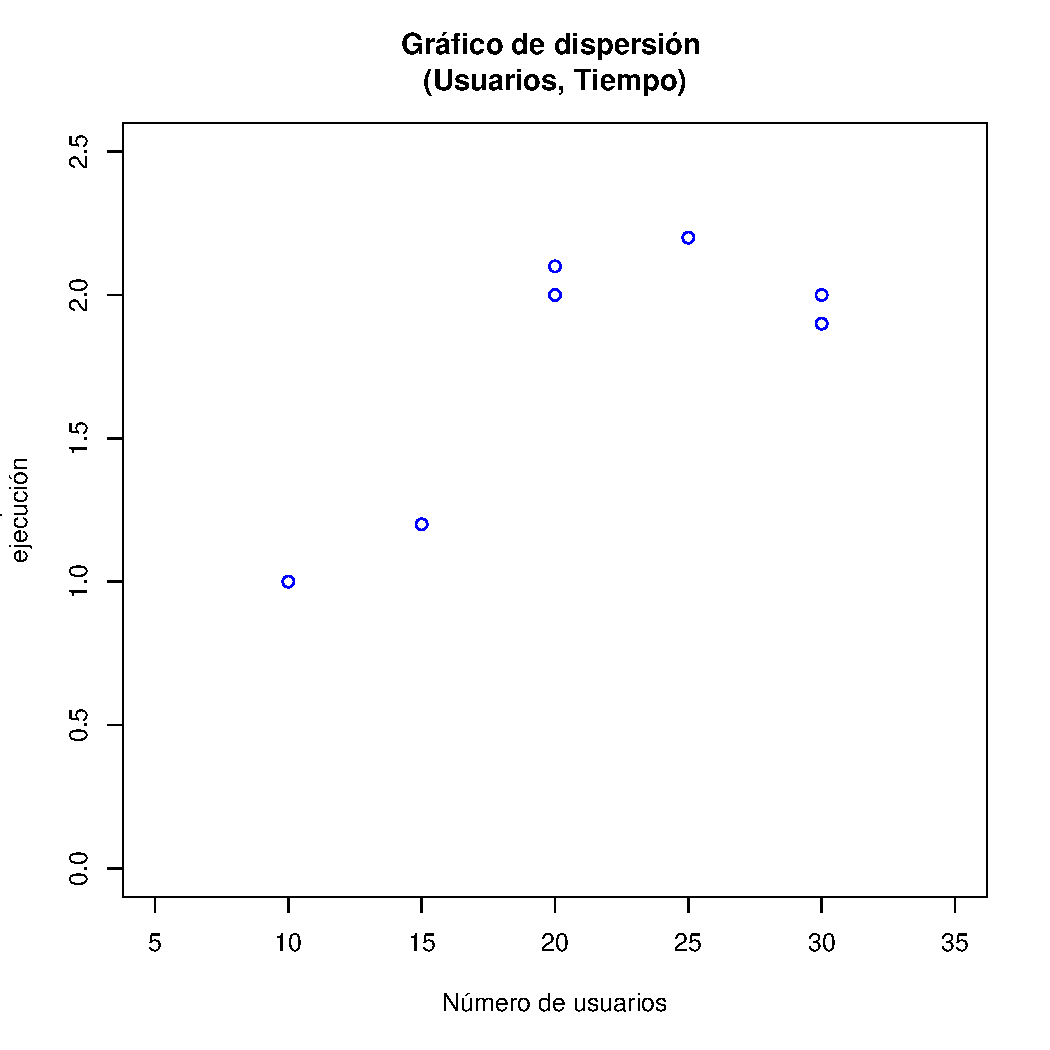
\includegraphics[width=\maxwidth]{figure/unnamed-chunk-9-1} 

\end{knitrout}

\item Para identificar un punto arbitrario, se procede de la siguiente manera: 

\begin{knitrout}
\definecolor{shadecolor}{rgb}{0.969, 0.969, 0.969}\color{fgcolor}\begin{kframe}
\begin{alltt}
\hlcom{# Sin cerrar la ventana del grafico anterior, ejecuta la siguiente instruccion}

\hlkwd{plot}\hlstd{(Usuarios, Tiempo,} \hlkwc{xlim}\hlstd{=} \hlkwd{c}\hlstd{(}\hlnum{5}\hlstd{,} \hlnum{35}\hlstd{),} \hlkwc{ylim}\hlstd{=} \hlkwd{c}\hlstd{(}\hlnum{0.0}\hlstd{,} \hlnum{2.5}\hlstd{),}
\hlkwc{type} \hlstd{=} \hlstr{"p"}\hlstd{,} \hlkwc{pch}\hlstd{=}\hlnum{1}\hlstd{,} \hlkwc{col} \hlstd{=} \hlstr{"blue"}\hlstd{,} \hlkwc{main} \hlstd{=} \hlstr{"Gráfico de dispersión 
(Usuarios, Tiempo)"}\hlstd{,} \hlkwc{xlab}\hlstd{=}\hlstr{"Número de usuarios"}\hlstd{,} \hlkwc{ylab}\hlstd{=}\hlstr{"Tiempo de 
ejecución"}\hlstd{)}

\hlkwd{identify}\hlstd{(Usuarios, Tiempo,} \hlkwc{n}\hlstd{=}\hlnum{1}\hlstd{)}
\end{alltt}
\end{kframe}
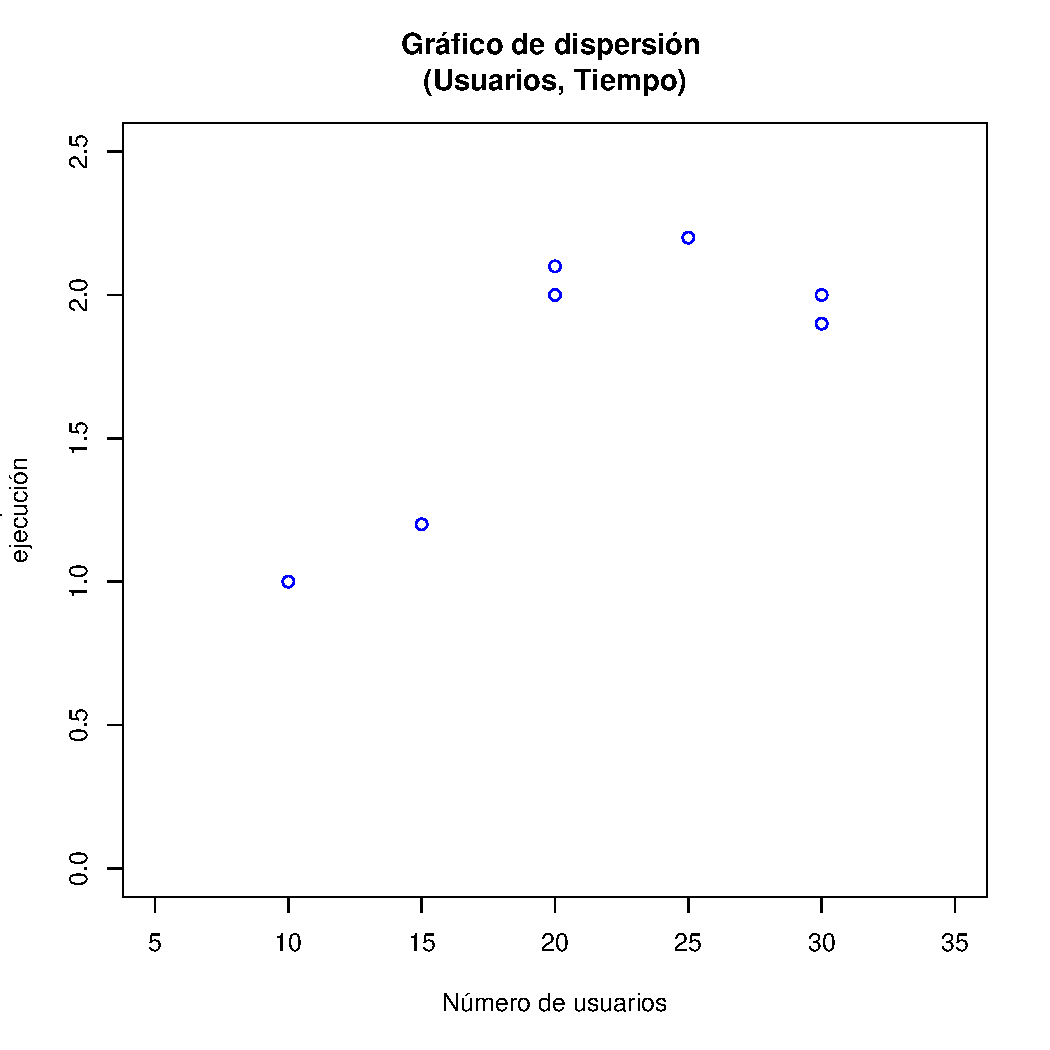
\includegraphics[width=\maxwidth]{figure/unnamed-chunk-10-1} 
\begin{kframe}\begin{verbatim}
## integer(0)
\end{verbatim}
\begin{alltt}
\hlcom{# n=1 indicaque solamente será un punto seleccionado }

\hlcom{# Y luego selecciona un punto en el grafico haciendo clic con el raton.}
\hlcom{# Esto es util para identificar puntos que podrian ser atipicos.}

\hlcom{# Debera aparecer en la R-Console el indice que corresponde a este punto. }
\end{alltt}
\end{kframe}
\end{knitrout}

\item Aplica la funci\'on lm() para encontrar el modelo lineal que se ajusta a los datos. 

\begin{knitrout}
\definecolor{shadecolor}{rgb}{0.969, 0.969, 0.969}\color{fgcolor}\begin{kframe}
\begin{alltt}
\hlstd{reg.Y.X} \hlkwb{<-} \hlkwd{lm}\hlstd{(Tiempo} \hlopt{~ -}\hlnum{1} \hlopt{+} \hlstd{Usuarios, Sistema,} \hlkwc{na.action}\hlstd{=}\hlkwa{NULL}\hlstd{,}
              \hlkwc{method}\hlstd{=}\hlstr{"qr"}\hlstd{,} \hlkwc{model}\hlstd{=}\hlnum{TRUE}\hlstd{)}

\hlcom{#-1 indica que no se toma en cuenta la constante en el modelo. }

\hlkwd{summary}\hlstd{(reg.Y.X)}
\end{alltt}
\begin{verbatim}
## 
## Call:
## lm(formula = Tiempo ~ -1 + Usuarios, data = Sistema, na.action = NULL, 
##     method = "qr", model = TRUE)
## 
## Residuals:
##     Min      1Q  Median      3Q     Max 
## -0.4831 -0.1873  0.2056  0.3127  0.5113 
## 
## Coefficients:
##          Estimate Std. Error t value Pr(>|t|)    
## Usuarios 0.079437   0.006496   12.23 1.82e-05 ***
## ---
## Signif. codes:  0 '***' 0.001 '**' 0.01 '*' 0.05 '.' 0.1 ' ' 1
## 
## Residual standard error: 0.3871 on 6 degrees of freedom
## Multiple R-squared:  0.9614,	Adjusted R-squared:  0.955 
## F-statistic: 149.5 on 1 and 6 DF,  p-value: 1.821e-05
\end{verbatim}
\begin{alltt}
\hlcom{# Note que es necesaria la instruccion anterior para poder visualizar los }
\hlcom{# resultados mas sobre salientes de la regresion encontrada. Nos muestra la}
\hlcom{# estimacion de los parametros junto con su significancia, el coeficiente de}
\hlcom{# determinacion. }
\end{alltt}
\end{kframe}
\end{knitrout}

\item Agrega la recta de regresi\'on al gr\'afico de dispersi\'on.

\begin{knitrout}
\definecolor{shadecolor}{rgb}{0.969, 0.969, 0.969}\color{fgcolor}\begin{kframe}
\begin{alltt}
\hlkwd{plot}\hlstd{(Usuarios, Tiempo,} \hlkwc{xlim}\hlstd{=} \hlkwd{c}\hlstd{(}\hlnum{5}\hlstd{,} \hlnum{35}\hlstd{),} \hlkwc{ylim}\hlstd{=} \hlkwd{c}\hlstd{(}\hlnum{0.0}\hlstd{,} \hlnum{2.5}\hlstd{),}
\hlkwc{type} \hlstd{=} \hlstr{"p"}\hlstd{,} \hlkwc{pch}\hlstd{=}\hlnum{1}\hlstd{,} \hlkwc{col} \hlstd{=} \hlstr{"blue"}\hlstd{,} \hlkwc{main} \hlstd{=} \hlstr{"Gráfico de dispersión 
(Usuarios, Tiempo)"}\hlstd{,} \hlkwc{xlab}\hlstd{=}\hlstr{"Número de usuarios"}\hlstd{,} \hlkwc{ylab}\hlstd{=}\hlstr{"Tiempo de 
ejecución"}\hlstd{)}

\hlkwd{abline}\hlstd{(reg.Y.X)}
\end{alltt}
\end{kframe}
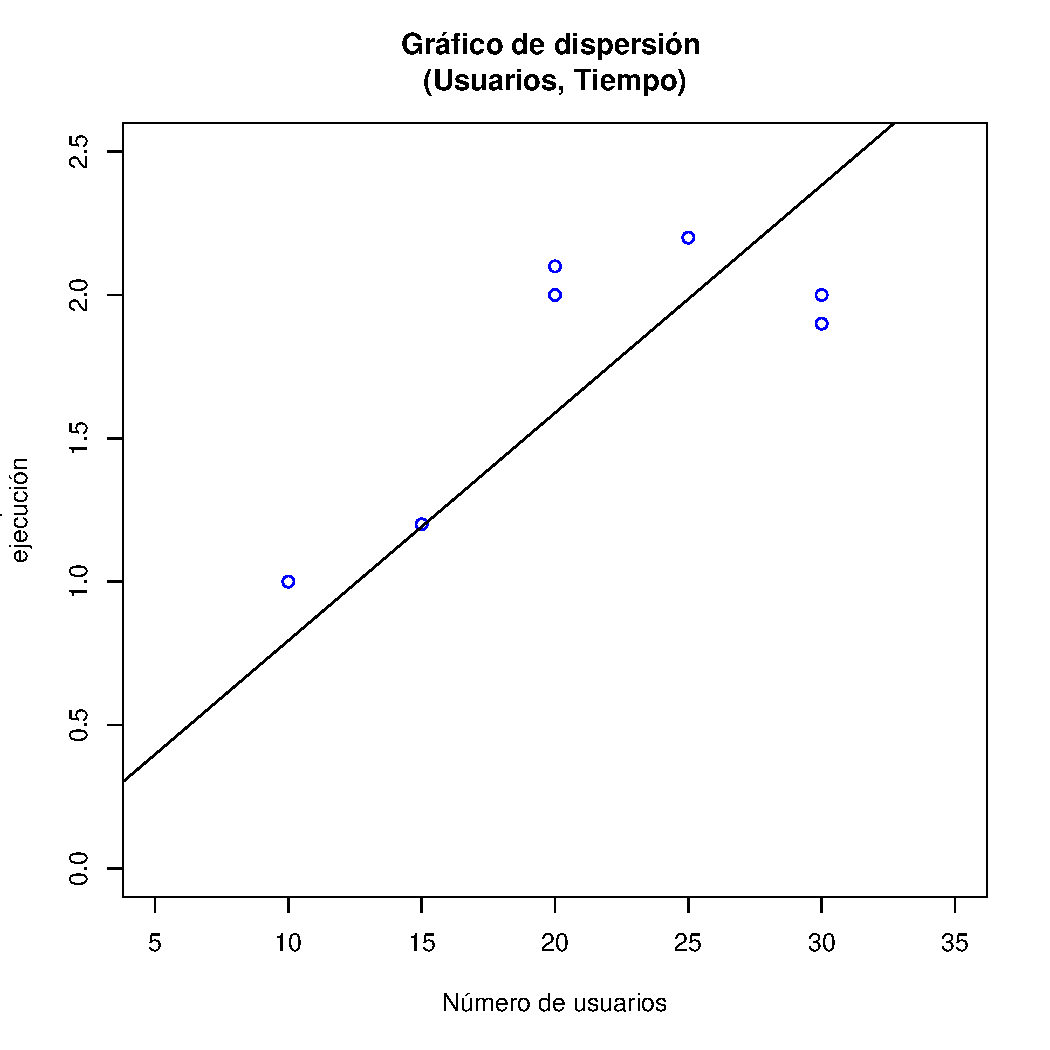
\includegraphics[width=\maxwidth]{figure/unnamed-chunk-12-1} 

\end{knitrout}

\textbf{Observaci\'on: Alternativamente si quiere una recta m\'as exacta use:}

\begin{knitrout}
\definecolor{shadecolor}{rgb}{0.969, 0.969, 0.969}\color{fgcolor}\begin{kframe}
\begin{alltt}
\hlkwd{line}\hlstd{(Usuarios,} \hlnum{0.079437}\hlopt{*}\hlstd{Usuarios)}
\end{alltt}
\begin{verbatim}
## 
## Call:
## line(Usuarios, 0.079437 * Usuarios)
## 
## Coefficients:
## [1]  0.2648  0.0662
\end{verbatim}
\end{kframe}
\end{knitrout}

\item Efect\'ua una an\'alisis de variabilidad del modelo o descomposici\'on de la varianza. 

\begin{knitrout}
\definecolor{shadecolor}{rgb}{0.969, 0.969, 0.969}\color{fgcolor}\begin{kframe}
\begin{alltt}
\hlstd{reg.anova} \hlkwb{<-} \hlkwd{anova}\hlstd{(reg.Y.X); reg.anova}
\end{alltt}
\begin{verbatim}
## Analysis of Variance Table
## 
## Response: Tiempo
##           Df  Sum Sq Mean Sq F value    Pr(>F)    
## Usuarios   1 22.4011 22.4011  149.53 1.821e-05 ***
## Residuals  6  0.8989  0.1498                      
## ---
## Signif. codes:  0 '***' 0.001 '**' 0.01 '*' 0.05 '.' 0.1 ' ' 1
\end{verbatim}
\end{kframe}
\end{knitrout}


  
  
  
  
  
  
  
  
  
  
  
  
  
\end{enumerate}


\end{document}
